% Created by tikzDevice version 0.12.3 on 2020-01-28 17:47:35
% !TEX encoding = UTF-8 Unicode
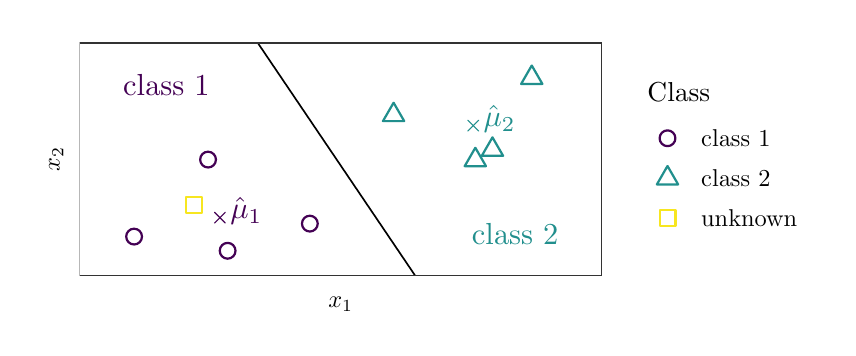
\begin{tikzpicture}[x=1pt,y=1pt]
\definecolor{fillColor}{RGB}{255,255,255}
\path[use as bounding box,fill=fillColor,fill opacity=0.00] (0,0) rectangle (289.08,108.41);
\begin{scope}
\path[clip] (  0.00,  0.00) rectangle (289.08,108.41);
\definecolor{drawColor}{RGB}{255,255,255}
\definecolor{fillColor}{RGB}{255,255,255}

\path[draw=drawColor,line width= 0.6pt,line join=round,line cap=round,fill=fillColor] (  0.00,  0.00) rectangle (289.08,108.41);
\end{scope}
\begin{scope}
\path[clip] ( 18.77, 18.77) rectangle (207.47,102.91);
\definecolor{fillColor}{RGB}{255,255,255}

\path[fill=fillColor] ( 18.77, 18.77) rectangle (207.47,102.91);
\definecolor{drawColor}{RGB}{68,1,84}

\path[draw=drawColor,line width= 0.8pt,line join=round,line cap=round] ( 72.25, 27.79) circle (  2.85);

\path[draw=drawColor,line width= 0.8pt,line join=round,line cap=round] ( 38.45, 32.92) circle (  2.85);

\path[draw=drawColor,line width= 0.8pt,line join=round,line cap=round] ( 65.18, 60.74) circle (  2.85);

\path[draw=drawColor,line width= 0.8pt,line join=round,line cap=round] (101.96, 37.60) circle (  2.85);
\definecolor{drawColor}{RGB}{33,143,141}

\path[draw=drawColor,line width= 0.8pt,line join=round,line cap=round] (161.76, 65.03) --
	(165.61, 58.37) --
	(157.92, 58.37) --
	(161.76, 65.03);

\path[draw=drawColor,line width= 0.8pt,line join=round,line cap=round] (167.95, 68.78) --
	(171.79, 62.12) --
	(164.10, 62.12) --
	(167.95, 68.78);

\path[draw=drawColor,line width= 0.8pt,line join=round,line cap=round] (182.15, 94.74) --
	(185.99, 88.08) --
	(178.31, 88.08) --
	(182.15, 94.74);

\path[draw=drawColor,line width= 0.8pt,line join=round,line cap=round] (132.22, 81.30) --
	(136.07, 74.64) --
	(128.38, 74.64) --
	(132.22, 81.30);
\definecolor{drawColor}{RGB}{247,230,32}

\path[draw=drawColor,line width= 0.8pt,line join=round,line cap=round] ( 57.20, 41.39) rectangle ( 62.91, 47.10);
\definecolor{drawColor}{RGB}{68,1,84}

\path[draw=drawColor,line width= 0.4pt,line join=round,line cap=round] ( 67.50, 37.80) -- ( 71.42, 41.72);

\path[draw=drawColor,line width= 0.4pt,line join=round,line cap=round] ( 67.50, 41.72) -- ( 71.42, 37.80);
\definecolor{drawColor}{RGB}{33,143,141}

\path[draw=drawColor,line width= 0.4pt,line join=round,line cap=round] (159.06, 71.06) -- (162.98, 74.98);

\path[draw=drawColor,line width= 0.4pt,line join=round,line cap=round] (159.06, 74.98) -- (162.98, 71.06);
\definecolor{drawColor}{RGB}{68,1,84}

\node[text=drawColor,anchor=base,inner sep=0pt, outer sep=0pt, scale=  1.10] at ( 78.99, 39.44) {$\hat{\mu}_1$};
\definecolor{drawColor}{RGB}{33,143,141}

\node[text=drawColor,anchor=base,inner sep=0pt, outer sep=0pt, scale=  1.10] at (170.55, 72.70) {$\hat{\mu}_2$};
\definecolor{drawColor}{RGB}{0,0,0}

\path[draw=drawColor,line width= 0.6pt,line join=round] ( 79.43,108.41) --
	(152.74,  0.00);
\definecolor{drawColor}{RGB}{68,1,84}

\node[text=drawColor,anchor=base west,inner sep=0pt, outer sep=0pt, scale=  1.10] at ( 34.47, 83.90) {class 1};
\definecolor{drawColor}{RGB}{33,143,141}

\node[text=drawColor,anchor=base east,inner sep=0pt, outer sep=0pt, scale=  1.10] at (191.78, 30.18) {class 2};
\definecolor{drawColor}{gray}{0.20}

\path[draw=drawColor,line width= 0.6pt,line join=round,line cap=round] ( 18.77, 18.77) rectangle (207.47,102.91);
\end{scope}
\begin{scope}
\path[clip] (  0.00,  0.00) rectangle (289.08,108.41);
\definecolor{drawColor}{RGB}{0,0,0}

\node[text=drawColor,anchor=base,inner sep=0pt, outer sep=0pt, scale=  0.88] at (113.12,  7.21) {$x_1$};
\end{scope}
\begin{scope}
\path[clip] (  0.00,  0.00) rectangle (289.08,108.41);
\definecolor{drawColor}{RGB}{0,0,0}

\node[text=drawColor,rotate= 90.00,anchor=base,inner sep=0pt, outer sep=0pt, scale=  0.88] at ( 11.56, 60.84) {$x_2$};
\end{scope}
\begin{scope}
\path[clip] (  0.00,  0.00) rectangle (289.08,108.41);
\definecolor{fillColor}{RGB}{255,255,255}

\path[fill=fillColor] (218.47, 26.81) rectangle (283.58, 94.87);
\end{scope}
\begin{scope}
\path[clip] (  0.00,  0.00) rectangle (289.08,108.41);
\definecolor{drawColor}{RGB}{0,0,0}

\node[text=drawColor,anchor=base west,inner sep=0pt, outer sep=0pt, scale=  0.99] at (223.97, 81.59) {Class};
\end{scope}
\begin{scope}
\path[clip] (  0.00,  0.00) rectangle (289.08,108.41);
\definecolor{fillColor}{RGB}{255,255,255}

\path[fill=fillColor] (223.97, 61.22) rectangle (238.43, 75.67);
\end{scope}
\begin{scope}
\path[clip] (  0.00,  0.00) rectangle (289.08,108.41);
\definecolor{drawColor}{RGB}{68,1,84}

\path[draw=drawColor,line width= 0.8pt,line join=round,line cap=round] (231.20, 68.45) circle (  2.85);
\end{scope}
\begin{scope}
\path[clip] (  0.00,  0.00) rectangle (289.08,108.41);
\definecolor{fillColor}{RGB}{255,255,255}

\path[fill=fillColor] (223.97, 46.76) rectangle (238.43, 61.22);
\end{scope}
\begin{scope}
\path[clip] (  0.00,  0.00) rectangle (289.08,108.41);
\definecolor{drawColor}{RGB}{33,143,141}

\path[draw=drawColor,line width= 0.8pt,line join=round,line cap=round] (231.20, 58.43) --
	(235.04, 51.77) --
	(227.36, 51.77) --
	(231.20, 58.43);
\end{scope}
\begin{scope}
\path[clip] (  0.00,  0.00) rectangle (289.08,108.41);
\definecolor{fillColor}{RGB}{255,255,255}

\path[fill=fillColor] (223.97, 32.31) rectangle (238.43, 46.76);
\end{scope}
\begin{scope}
\path[clip] (  0.00,  0.00) rectangle (289.08,108.41);
\definecolor{drawColor}{RGB}{247,230,32}

\path[draw=drawColor,line width= 0.8pt,line join=round,line cap=round] (228.35, 36.68) rectangle (234.05, 42.39);
\end{scope}
\begin{scope}
\path[clip] (  0.00,  0.00) rectangle (289.08,108.41);
\definecolor{drawColor}{RGB}{0,0,0}

\node[text=drawColor,anchor=base west,inner sep=0pt, outer sep=0pt, scale=  0.88] at (243.38, 65.42) {class 1};
\end{scope}
\begin{scope}
\path[clip] (  0.00,  0.00) rectangle (289.08,108.41);
\definecolor{drawColor}{RGB}{0,0,0}

\node[text=drawColor,anchor=base west,inner sep=0pt, outer sep=0pt, scale=  0.88] at (243.38, 50.96) {class 2};
\end{scope}
\begin{scope}
\path[clip] (  0.00,  0.00) rectangle (289.08,108.41);
\definecolor{drawColor}{RGB}{0,0,0}

\node[text=drawColor,anchor=base west,inner sep=0pt, outer sep=0pt, scale=  0.88] at (243.38, 36.51) {unknown};
\end{scope}
\end{tikzpicture}
